\documentclass[12pt,a4paper,twoside,openany]{jbook}
\usepackage{master}
\usepackage{udline}
\usepackage{booktabs}
\usepackage{multirow}

\usepackage[dvipdfmx]{graphicx}
%\usepackage[dvipdfmx]{color}
\usepackage{bm}
\usepackage{amsmath}
\usepackage{ascmac}

\usepackage[usenames]{color}
\newcommand\mychangecolor[1]{\textcolor[rgb]{1,0,0}{\textbf{#1}}}
\usepackage{fancyvrb}
\usepackage{comment}
\bachelor
\title{計算量を考慮した対話行為設計に基づく強化学習による発話選択
}
\supervisor{駒谷 和範 教授}
\affi{大阪大学工学部 電子情報工学科}
\author{黒田 佑樹}

\pagestyle{headings}

\begin{document}
\maketitle
\clearpage

\pagenumbering{roman}
\setcounter{page}{1}

%\input{abstract}
\atitle{計算量を考慮した対話行為設計に基づく強化学習による発話選択
}
\abstracttext{

%背景・目的
近年,特定の目標を持たない非タスク指向型対話システムに注目が集まっている.
非タスク指向型対話の中にユーザの話の聞き役となり,ユーザの話したいという欲求を満たす傾聴型対話システムがある.
傾聴型対話システムでは,システムが話の流れに合わない発話を出力すると,ユーザは気持ちよく対話を続けることができない.



そこで本研究では強化学習を用いて,破綻の生じにくい発話選択の戦略の獲得を目指す.
強化学習を用いて発話選択の戦略を獲得するには,対話の状態をどのように表現するか,どのような単位で行動を設計するかが重要となる.

%問題点
発話選択の戦略獲得に強化学習を用いる際,行動の設計としては大きく2つの方針がある.
%強化学習を用いた発話選択には様々な設計手法がある.
一点目は,最もシンプルに,発話全てを行動とする手法である.しかし,この手法では,用いる発話の数によっては探索すべき空間が増加し,計算量も増加する.
二点目は,発話集合を特徴ごとに分類して行動とする方法である.しかし,この方法では,同じクラスに分類された発話のうち,どれが選択されるかをコントロールできず,破綻が生じることがある.実際,発話集合を対話行為に分類して行動とした従来手法では,対話行為選択以降の発話選択がランダムであるため,破綻が生じることが多かった.



%やったこと
本研究では,対話行為の一部のみを詳細化して行動とすることで,計算量を増やしすぎず,破綻の生じる発話の出力を防ぐ.アプローチとしては,対話行為を行動として強化学習を行ったうえで,対話行為内からランダムに発話を選択する従来手法を拡張する.
まず,従来手法に基づくシステムにおいて,破綻の生じやすい対話行為の順番を分析した.
次に,それに含まれる対話行為を詳細化して,そのまま状態と行動の設計に用いる.
これによってより細かい行動が表現できるようになり,対話行為内からランダムに発話が選択されることがなくなる.
また,設計した状態と行動の組み合わせに関して,負の報酬を設計する.
これによって,ある状態で,破綻が生じる行動の出力を防ぐことができる.
これらの状態と行動と報酬の設計によって,対話行為内の発話に優先順位がつけられ,破綻の生じない発話を選択しやすくなる.



%実験手法と結果
実験では,破綻の生じにくさと計算時間の2つの観点から提案手法を評価した.
比較する手法としては,提案手法,対話行為を行動とした手法,発話全てを行動とした手法の3つを用いた.
破綻の生じにくさに関する評価実験では,3つの手法で対話を行い,比較した.
結果として,破綻の割合が提案手法では5\%,対話行為を行動とした手法で17\%,発話全てを行動とした手法で6.5\%であった.これにより,提案手法は破綻の生じにくさにおいて,対話行為を行動とした手法よりも優れており,発話全てを行動とした手法と同程度の性能を実現していることが示された.
また,計算量に関する評価実験では,3つの手法に関して,探索空間のサイズに比例するエピソード数で学習を行い,そのときにかかる時間によって評価を行った.
結果として,学習を行ったときにかかる時間が提案手法では2777秒,発話全てを行動とした手法で6118秒であった.これにより,提案手法では,破綻の生じやすさに関して同程度の性能をもつ,発話全てを行動とする手法よりも計算時間を削減できていることが示された.

}

\abstractpage
\tableofcontents
\cleardoublepage

\pagenumbering{arabic}
\setcounter{page}{1}

%
\newcommand{\argmin}{\mathop{\rm arg~min}\limits}


%%%%% 1章 %%%%%%%%%%%%%%%%%%%%%%%%%%%%%%%%%%%%%%%%%%%%%%%%%%%%%%%%%%%%%%%
\chapter{序論}
%\section{背景と目的}
%非タスク指向型対話システムについて
対話システムはタスク指向型と非タスク指向型に大別される.
タスク指向型対話システムとは,対話を通して特定の目標を達成するためのシステムのことである.
タスク指向型対話システムの例としては,ユーザの情報収集を助けるシステム等\cite{saruwatari}がある.
一方,非タスク指向型の例としては,ユーザと対話を続けること自体を目的とした雑談対話システムがある.

%傾聴型対話システムについて
非タスク指向型対話システムの中でも,ユーザの話の聞き役となるものを傾聴対話システム\cite{meguro}\cite{ishida}と呼ぶ.
傾聴対話システムはユーザの話したい,聞いてほしいという欲求を満たすことが期待される.

%雑談対話システムについて


%傾聴(雑談)対話システムにおける問題点
傾聴対話システムではユーザに気持ちよく話してもらうために,話の流れに合った質問をしたり,反応を返したりする必要がある.
システムがこれらを行った時,話の流れに合わない,不自然な発話を返してしまうことがある.これを破綻と呼ぶ.
対話中に破綻が生じれば,ユーザは対話自体に違和感を感じ,気持ちよく対話を続けることができない.
そのため,破綻しない発話を出力することが重要である.

%傾聴(雑談)対話システムにおける発話生成方法
システム発話を出力するためのアプローチには主に,ルールベース,生成ベース,用例ベースの3つが存在する\cite{python}.
ルールベースとはユーザの入力発話に対するシステム応答をルール形式で記述するアプローチである.
生成ベースとは単語や文字レベルからニューラルネットワーク等を用いてシステム応答を生成するアプローチである.
用例ベースとは予め用意された発話候補からシステム応答を選択するアプローチである.
傾聴対話におけるユーザの発話は多様であり,ルールベースではルールの記述が膨大になるため,適していない.
また,生成ベースでは,単語や文字レベルから応答を生成するため,出力したシステム発話そのものが破綻してしまう場合がある.
そこで,本研究では,一つの応答を複数の文脈に使え,かつシステム発話そのものが破綻することのない,用例ベースのアプローチに着目する.

%強化学習を用いた対話システム
対話システムでの適切な応答選択のための戦略はしばしば強化学習で定式化される.
強化学習とは機械学習の1種で,ある状態である行動をとる価値を,対象のタスクの試行を通して更新していき,最適な方策を学習する手法である.
強化学習は試行錯誤を繰り返してより良い方策を学習するという性質上,対話システムに適している.

%強化学習を用いた発話選択手法
強化学習は用例ベースの対話システムに用いられることがある.
用例ベースを用いた対話システムを強化学習で定式化する場合,最もシンプルな方法として,全ての発話をそのまま行動とするものがある.しかし,この方法では,全体の発話集合の数によっては,探索すべき空間が膨大になってしまう.

これを解決するための方法として,発話候補の集合を行動とする強化学習の設計がある.
この方法では,同一行動とみなされる発話候補内の発話は,ある状況において,どれを選んでも適切である必要がある.
そのため,特徴ごとに発話を分類して状態や行動の設計に用いる.
しかし,集合中からどれを選んでも破綻が生じない発話集合を設計することは困難である.実際に,発話集合を対話行為単位に分類して行動とし,その中からランダムに発話を選ぶ従来手法\cite{nishimoto2}では,対話に破綻が生じてしまうことがあった.



%本研究での発話選択手法
本研究では,全ての発話を行動にした手法よりも計算量が少なく,また,発話集合を対話行為単位に分類して行動とした手法よりも破綻の生じにくい対話システムの構築を目指す.
そのために,対話行為を行動とし,行動の中から発話をランダムに選ぶ手法\cite{nishimoto2}をベースとしたアプローチを提案する.提案手法では,この手法の破綻しやすい対話行為の順番を分析し,そこに現れる対話行為内の発話のみを詳細化して状態や行動の設計に用いる.
これにより,計算量が増えすぎることなく,同一対話行為内の発話を個々に選択できるようになり,破綻が減少することが期待される.

%章構成
以下に本論文の章構成を示す.
%1.2節では本研究で提案する発話選択手法に関する他の研究をとりあげ,本研究の位置づけを確認する.
2章では強化学習を用いた発話選択手法と,その問題点について述べる.
3章では強化学習を用いた発話選択手法の問題点を解決するための,本研究での提案手法の方針と詳細を述べる.
4章では提案手法を用いた対話を,破綻の生じやすさと計算量の観点から評価を行い,提案手法の問題点解決への有効性を示す.
5章では本研究のまとめと今後の課題について述べる.
\begin{comment}
%\section{関連研究}\label{kanren}
本節では対話システムにおける破綻削減や強化学習を用いた対話システムに関連する研究を述べ,本研究の位置づけを確認する.

%破綻に関する研究
%強化学習を用いた対話システム
強化学習を用いた対話システムでは,対話の状態に応じてシステム行動を選択し,報酬を与えるというサイクルで探索を行い,ある対話状態での行動選択方針を学習する.

システム行動を応答生成モジュールとした例として江頭らの研究\cite{egashira}がある.
これは「ニュース記事中の一文を表示する」,「Wikipedia定義文の検索を行う」などの応答生成モジュールを作成し,その選択方策を強化学習によって学習するものである.本研究では発話や発話集合そのものを行動として強化学習を行う.
%対話破綻に関する研究


%強化学習を用いた発話選択手法の概要(2章でもいい?)
強化学習を用いた発話選択では,対話の状態を表現し,その状態で適切なシステム発話を選択する方策を学習する.
状態表現にはユーザ発話の音声情報,また,システム発話の言語情報等を用いる.
行動表現にはシステム発話あるいはその集合を用いる.
これらを踏まえて,強化学習を用いた発話選択では,まず発話集合を適切に分類する必要がある.


%対話行為に分類した研究
発話集合を対話行為単位で分類した例として西本らの研究\cite{nishimoto}がある.
この研究では心象等新たな特徴量を用いることで,発話集合を新たな対話行為に分類することによって破綻を防いだ.
本研究では,この対話行為をさらに細かくすることで,より多くの破綻を防ぐ.

%発話全部を状態行動とした研究
発話集合を発話単位で分類して強化学習を行った研究として佐藤らの研究\cite{satoh}がある.
この研究では発話単位で状態行動を設計して強化学習を行い,発話選択戦略を獲得した.
計算量を削減するための試みとして深層強化学習を用いる点が本研究とは異なる.
\end{comment}
%%%%% 2章 %%%%%%%%%%%%%%%%%%%%%%%%%%%%%%%%%%%%%%%%%%%%%%%%%%%%%%%%%%%%%%%
\chapter{強化学習を用いた発話選択手法とその問題点}
本章では\ref{kyoka}節で,本研究で扱う強化学習と,その手法の1種であるQ学習について,基本的な知識を説明する.
%\ref{kyoka_hatuwa}節では,強化学習を用いた対話システムの中でも,発話選択に関するものについて説明する.
\ref{kanren}節では強化学習を用いた対話システムに関する研究を述べ,本研究の立ち位置を確認する.
%\ref{baseline1}節では強化学習の状態や行動の設計に,発話をそのまま用いた例を紹介する.
%\ref{baseline2}節では強化学習の状態や行動の設計に対話行為を用いた既存手法を紹介する.
\ref{baseline2}節では,発話集合を特徴ごとに分類して行動とする強化学習の設計の中でも,対話行為を用いた従来手法を紹介する.
\ref{bunseki}節では対話行為を行動とした従来手法の問題点を分析する.
%\ref{kyoka}節では既存手法を理解するために必要な強化学習の基本的な知識を説明する.

\section{強化学習とは}\label{kyoka}
%強化学習の概要
強化学習とは機械学習の学習方法の1種である.行動によって報酬が得られる「環境」を与えて,各状態において報酬につながる行動が出力されるようにモデルのパラメータを調整する.
学習されたモデルは,状態を入力として,とるべき行動を出力する「方策」とみなせる.
学習は何回かの行動を1まとまりとしたエピソード単位で行われる.

%MDP
強化学習では,マルコフ性に従う環境であるマルコフ決定過程(MDP)を仮定して学習を行うことが多い.
マルコフ性とは,遷移先の状態が直前の状態と行動にのみ依存し,報酬が直前の状態と遷移先に依存するというものである.
MDPは以下の4つの要素で構成される.
\begin{itemize}
\item s: 状態
\item a: 行動
\item T: 状態と行動を引数に,次の状態と遷移確率を出力する関数
\item R: 状態と遷移先を引数に,報酬を出力する関数
\end{itemize}
MDPを仮定した強化学習は図\ref{MDP}のように表される.
\begin{figure}[ht]
  \begin{center} %センタリングする
    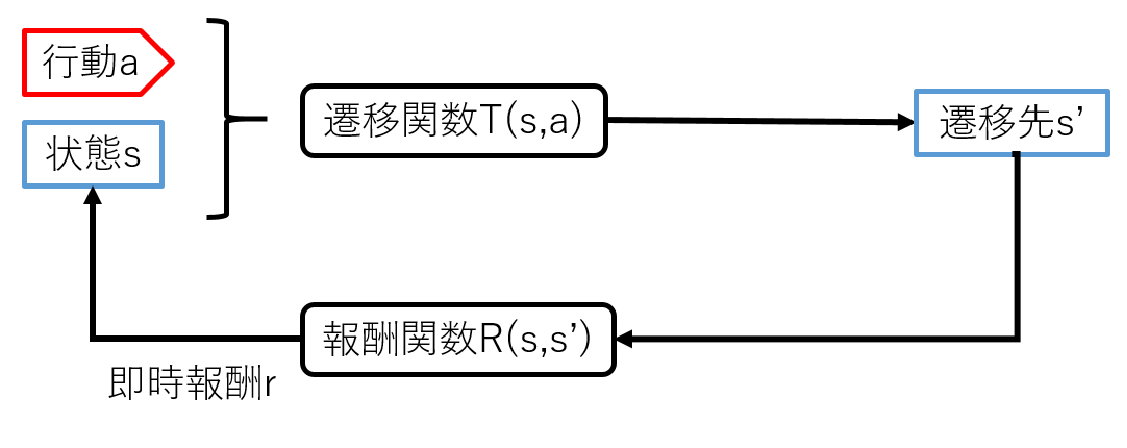
\includegraphics[width=12cm]{MDP.eps}
    \caption{MDPを仮定した強化学習} %タイトルをつける
    \label{MDP} %ラベルをつけ図の参照を可能にする
  \end{center}
\end{figure}

%モデルベースとモデルフリー
強化学習にはモデルベースとモデルフリーの手法が存在する.
前者は状態遷移関数や報酬関数が既知であり,後者は未知である.
後者では遷移関数が分かっていないため,初めはランダムに行動選択を行い,報酬を得ることで,より高い報酬が得られる状態遷移方法を経験的に知る.ある程度の経験が得られたら,これを仮の遷移関数として学習を行う.これをEpsilon-Greedy法という.

%モンテカルロ法とTD法
%モデルフリーの手法での遷移関数の更新方法としてTD法とモンテカルロ法がある.
%前者では行動ごとに遷移関数を更新するが,後者は1エピソードごとに更新する.

%Q学習
モデルフリーの強化学習として,Q学習がある.
本研究で扱うシステムでは強化学習の手法としてこのQ学習を用いている.
Q学習ではある状態である行動をとる価値を学習する.
この価値をQ値という.
Q学習の価値更新方法は下記の式\ref{Q}に従う.
\begin{equation}
\label{Q}
Q(s_t,a_t) \leftarrow Q(s_t,a_t) + \alpha(r_{t+1} + \gamma Q(s_{t+1},s_{t+1}) - Q(s_t,a_t))
\end{equation}
設定された即時報酬$r_{t+1}$と遷移先の価値$Q(s_{t+1})$に割引率$\gamma$をかけたものの和によって,その状態行動セットの新たな価値が更新される.
更新の速度は学習率$\alpha$によって決定される.
ある状態である行動をとる価値を記述した表が遷移関数に対応するものであり,Qテーブルと呼ばれる.
状態数と行動数の組み合わせの数がこのQテーブルのサイズとなる.


%強化学習の対話システムへの応用
%強化学習を用いた対話システムは行動を何にするかによって大別される.
%本研究ではシステム発話自体の選択に強化学習を用いる.

\begin{comment}
%\section{強化学習を用いた対話システムと発話選択}\label{kyoka_hatuwa}
強化学習を用いた対話システムでは,対話の状態に応じてシステム行動を選択し,報酬を与えるというサイクルで探索を行い,ある対話状態での行動選択方針を学習する.

本研究では発話もしくは発話集合をシステム行動として,発話選択の方策を学習し,破綻の少ない対話を目指す.
%強化学習を用いた発話選択では,対話の状態を表現し,その状態で適切なシステム発話を選択する方策を学習する.
%状態表現にはユーザ発話の音声情報,また,システム発話の言語情報等を用いる.

本研究では主にシステム発話の言語情報に注目する.
%発話を選択するアプローチである以上,当然行動表現にはシステム発話あるいはその集合が用いられる.
適切なシステム発話の選択を行うためには,これら状態,行動を適切に設計する必要がある.
\end{comment}

\section{強化学習を用いた対話システムの関連研究}\label{kanren}
本節では強化学習を用いた対話システムに関連する研究を述べ,本研究の位置づけを確認する.

%強化学習を用いた対話システムでは,対話の状態に応じてシステム行動を選択し,報酬を与えるというサイクルで探索を行い,ある対話状態での行動選択方針を学習する.
%破綻に関する研究
%強化学習を用いた対話システム

強化学習のシステム行動を応答生成モジュールとした対話システムとして,江頭らの研究\cite{egashira}がある.
これは「ニュース記事中の一文を表示する」,「Wikipedia定義文の検索を行う」などの応答生成モジュールを作成し,その選択方策を強化学習によって学習するものである.
本研究では発話や発話集合そのものを行動として強化学習を行う点が違う.

発話や発話集合そのものを行動とする手法で,最もシンプルなものが,全ての発話を行動とする方法である.しかし,この方法では全体の発話数が多くなった時に,探索すべき空間が爆発的に増えてしまう.
佐藤ら\cite{satoh}は発話単位で行動を設計して強化学習を行い,発話選択の戦略を獲得した.
この研究では,深層強化学習を用いることで,探索すべき空間の爆発に対処した.
一方,本研究ではQ学習を用い,状態と行動の数を発話分類の工夫によって削減することで,探索空間の増加に対処する.

また,探索空間を増やし過ぎないために考案された方法として,発話集合を何らかの特徴ごとに分割して行動とするものがある.これにより,発話数がいくら増えようが,行動数は分類した数より多くなることはない.
Yuら\cite{yu}は発話集合を「ジョーク」や「話題の変更」等に分類して行動設計を行った.
本研究では,このような特徴ごとに分類した行動の一部の中身を発話レベルまで詳細化して行動とし,出力の際の優先順位を強化学習することで,意図しない発話の出力を防ぐ.
具体的には,\ref{baseline2}節で詳述する,発話集合を対話行為に分類して行動とする従来手法をベースとする.


\begin{comment}
発話や発話集合そのものを行動として扱う場合,全ての発話の集合をどのような単位に分類するのかが重要になる.
システムは分類された発話集合の単位でしか行動することができないため,分類が粗すぎると,状況に合わない不適切な発話を選択してしまう.一方,分類を細かくし過ぎると,行動数が増え計算量も増加する.

%対話行為に分類した研究
発話集合を対話行為単位で分類して行動設計を行った例として,西本らの研究\cite{nishimoto}がある.
この研究では心象等新たな特徴量を用いて,発話集合を新たな対話行為に分類することによって破綻を防いだ.
本研究では,この対話行為をさらに細かくすることで,より多くの破綻を防ぐ.

%発話全部を状態行動とした研究
発話集合を発話単位で分類して強化学習を行った研究として佐藤らの研究\cite{satoh}がある.
この研究では発話単位で行動を設計して強化学習を行い,発話選択戦略を獲得した.
計算量を削減するための試みとして深層強化学習を用いる点が本研究とは異なる.
\end{comment}
\begin{comment}
%\section{発話そのものを行動とする設計}\label{baseline1}
最もシンプルな強化学習の設計として,システム発話集合中の発話をそのまま状態,行動とするものが考えられる.

%本研究ではこの手法をベースライン手法1と呼ぶ.
%例えば,あるシステム発話を選択した後にこのシステム発話がくるのはおかしい,というような関係に負の報酬を設定して,Q学習を行うと,適切なシステム発話選択方法が学習できそうである.
しかし,この方法でQ学習を行ったとすると,Qテーブルのサイズが発話数$\times$発話数になってしまい,全体の発話数によっては探索すべき空間が爆発的に増える.
\end{comment}

\section{対話行為を単位とする行動設計}\label{baseline2}
\ref{kanren}節で述べた,発話全てを行動とした際の探索空間の増加への対応である,発話集合を特徴ごとに分類して行動とする方法の1例を詳しく紹介する.
%発話集合をなんらかの単位に分類して状態行動設計に用いれば,発話そのものを行動とするよりも報酬の設定にかかるコストや状態行動数を削減することができる.
西本ら\cite{nishimoto2}は発話集合を対話行為に分類して行動とする手法を用いた.
%本研究ではこの手法をベースライン手法2と呼ぶ.
以下にその手法の状態と行動の設計を示す.

%発話集合
\begin{comment}
用いる発話集合は,雑談対話コーパスHazumi1902\cite{hazumi}から話題「スポーツ」「音楽」「食事」「旅行」の4つの話題で用いられる発話に,どの話題にも使用可能な「default」発話を加えた117発話である.
\end{comment}

%行動設計
この手法ではシステム発話集合を,表\ref{taiwakoui}に示した8つの対話行為に分類したものを行動として扱う.
表中の対話行為の記号は表\ref{yougo}に示した用語の組み合わせで表現されている.
西本らの研究では,雑談対話コーパスHazumi1902\cite{hazumi}から話題「スポーツ」「音楽」「食事」「旅行」の4つの話題で用いられる発話に,どの話題にも用いられる「default」の発話を加えた発話集合を用いている.表\ref{yougo}の「特定話題」は,前者の4つの話題に属する発話で構成される発話集合であることを示しており,「default」は後者の「default」発話に属する発話で構成される発話集合であることを示している.
\begin{table}[tb]
    \caption{対話行為8種類}\label{taiwakoui}
    \centering
    \begin{tabular}{|l|l|}\hline 
         対話行為&説明  \\ \hline \hline
         qs\_o\_d&(a)指示語あり質問(default) \\ \hline
         qs\_o\_s&(b)指示語あり質問(特定話題) \\ \hline
         qs\_x\_s&(c)指示語なし質問(特定話題) \\ \hline
         re\_o\_m&(d)指示語あり応答(特定話題+default) \\ \hline
         re\_x\_d&(e)指示語なし応答(default) \\ \hline
         re\_x\_m&(f)指示語なし応答(特定話題+default) \\ \hline
         thank&(g)感謝 \\ \hline
         io&(h)情報提供 \\ \hline
    \end{tabular}
\end{table}

%状態設計
この手法では状態を以下の3つの要素の組み合わせによって表現する.
\begin{enumerate}
\item 簡易対話行為(表\ref{kani}): 4状態
\item ユーザ発話に特定名詞が含まれるかどうか: 2状態
\item ユーザ心象: 3状態
\end{enumerate}
簡易対話行為は,発話集合を,行動として設計された8つの対話行為よりさらに粗く分類したものである.
ユーザ発話に特定名詞が含まれるかという状態は,ユーザ発話に特定名詞が含まれれば指示語あり応答を返したいという思想のもと設計された状態である.
また,ユーザ心象はユーザが今現在対話を面白いと思っているかどうかを3段階で表している.
この値はユーザ入力によって取得されるものとする.
これらの組み合わせ4$\times$2$\times$3の合計24状態がこの手法での状態空間となる.

\begin{table}[tb]
    \caption{簡易対話行為}\label{kani}
    \centering
    \begin{tabular}{|l|l|}\hline 
         対話行為&説明  \\ \hline \hline
         qs&質問 \\ \hline
         re&応答 \\ \hline
         io&情報提供 \\ \hline
         ct&話題変更 \\ \hline

    \end{tabular}
\end{table}
\begin{table}[tb]
    \caption{用語説明}\label{yougo}
    \centering
    \begin{tabular}{|l|l|}\hline 
         用語&説明  \\ \hline \hline
         qs&質問(question) \\ \hline
         re&応答(response) \\ \hline
         io&情報提供() \\ \hline
         ct&話題変更(change theme) \\ \hline \hline
        o&指示語あり \\ \hline
        x&指示語なし \\ \hline \hline
        s&特定話題(specific) \\ \hline
        d&デフォルト話題(default) \\ \hline
        m&特定話題+デフォルト話題(mix) \\ \hline
        
    \end{tabular}
\end{table}


%報酬設計
\begin{comment}
報酬設計は以下のとおりである.
\begin{enumerate}
    \item ユーザ心象値(単一)(+1, 0, -1)
    \item ユーザ心象値(連続)(+5, 0, -5)
    \item 簡易的なシステム対話行為の連続性 (+0 ~ +10)
    \item 特定の名詞を含むユーザ発話に対するシステム行動 (+10, 0, -10)
    \item システム行動「thank」の選択 (0, +10)
\end{enumerate}
報酬1は心象が低ければ+1の報酬,高ければ-1の報酬をつける.
報酬2は心象が3連続で高ければ+5,低ければ-5の報酬をつける.
報酬3は簡易対話行為の連続性に人手で+1から+10の報酬をつける.
報酬4はユーザ発話に特定名詞(固有名詞等)が含まれる場合に,指示語ありの対話行為を選べば+10,含まれない場合に選べば-10の報酬をつける.
報酬5は話題変更の前に感謝の対話行為が選ばれた場合,+10の報酬をつける.
\end{comment}

\section{対話行為を単位とする行動設計の問題点}\label{bunseki}
対話行為を単位とする行動設計では,システムは対話行為単位でしか発話選択ができない.そのため,対話行為単位での適切な発話選択は可能であるが,発話の具体的な内容までは考慮できず,破綻の生じる発話を選択してしまうことが考えられる.

この手法を実装して,システムと対話を行ったところ,実際にユーザ発話と次のシステム発話がかみ合わない例が見られた.これらを分析した結果,以下の3パターンのような順番で対話行為が選択された時に,破綻が生じやすかった.
\begin{screen}
\begin{verbatim}
【パターン1】
                   指示語なし質問 
                         ↓
 指示語あり質問(特定話題) or 指示語あり質問(default)
\end{verbatim}
\end{screen}
\begin{screen}
\begin{verbatim}
【パターン2】
      指示語あり質問(特定話題) or 指示語なし質問 
                         ↓
               指示語あり応答 or 感謝
\end{verbatim}
\end{screen}
\begin{screen}
\begin{verbatim}
【パターン3】
                指示語あり質問(default)
                          ↓
                指示語あり応答 or 感謝
\end{verbatim}
\end{screen}

以下で3つのパターンについて破綻例を交えながら説明を行う.破綻例の赤字は破綻を表しており,Sはシステムの発話であること,Uはユーザの発話であることを表している.システム発話に添えられた記号は対話行為を表す.
\subsection*{パターン1}%:\\ {\small 指示語なし質問 → 指示語あり質問(特定話題) or 指示語あり質問(default)}}


パターン1の破綻は,システムが指示語なし質問をしたときのユーザの応答に対して,指示語ありの質問を重ねてしたときに生じる破綻である.
例を図\ref{pattern1}に示す.ここでは,S1で「スポーツをする目的は何ですか?」と尋ねていて,U1ではユーザがスポーツをする目的について答えることが予測できる.しかし,S2では「そのスポーツ」と言って,急に特定のスポーツの話の指示語あり質問(qs\_o\_s)が選択されていて,破綻が生じている.

パターン1では選択された対話行為内に相応しい発話があるにも関わらず,破綻が生じている.
図\ref{pattern1}の例でも,S2で選ばれた特定話題の指示語あり質問(qs\_o\_s)の中には,「そのほか健康のために、気を付けていることはありますか?」等相応しい発話が他にある.それにも関わらず,ここでは,「そのスポーツのおすすめポイント~」が選ばれてしまっている.これは,ベースライン手法2では行動が対話行為単位であるため,特定話題の指示語あり質問(qs\_o\_s)に属する発話集合の中からランダムに発話が選ばれてしまっているためである.このことは,S2がデフォルト話題の指示語あり質問(qs\_o\_d)のときにも同様に言える.


\begin{figure}[tb]
\begin{screen}
\centering
\begin{Verbatim}[commandchars=\\\{\}]
S1:  スポーツをする目的は何ですか?(qs_x_s)
U1: 健康増進のためですかね
\mychangecolor{S2(破綻): そのスポーツのおすすめポイントを教えてください(qs_o_s)}
U2: どのスポーツ? 
\end{Verbatim}
\end{screen}
\caption{パターン1の破綻例}
\label{pattern1}
\end{figure}


\subsection*{パターン2}%: \\{\small 指示語あり質問(特定話題) or 指示語なし質問 \\\hspace{2pc}→ 指示語あり応答 or 感謝}}


パターン2の破綻は,システムが指示語あり質問(特定話題)もしくは指示語なし質問をしたときのユーザ応答に対して,指示語ありの応答や感謝を返したときに生じる破綻である.
例として図\ref{pattern2}を示す.ここでは,S1で「競技は何をご覧になりますか?」と尋ねていて,U1ではユーザが特定のスポーツを答えることが予測できる.それにも関わらず,S2では「それは大変ですよね」という,違和感のある指示語あり応答(re\_o\_m)を返してしまっている.

パターン2では選択された対話行為内に相応しい発話があるにも関わらず,破綻が生じている.
図\ref{pattern2}の例でも,S2で選ばれた特定話題の指示語あり応答(re\_o\_m)の中には,「なるほど、面白そうですね。機会があれば私も見てみたいです!」等相応しい発話が他にある.それにも関わらず,ここでは,「それは大変ですよね」が選ばれてしまっている.これは,ベースライン手法2では行動が対話行為単位であるため,指示語あり応答(re\_o\_m)に属する発話集合の中からランダムに発話が選ばれてしまっているためである.このことは,S1が特定話題の指示語あり質問(qs\_o\_s)であるときや,S2が感謝(thank)であるときにも同様に言える.

\begin{figure}[tb]
\begin{screen}
\centering
\begin{Verbatim}[commandchars=\\\{\}]
S1: 競技は何をご覧になりますか?(qs_x_s)
U1: 野球です
\mychangecolor{S2(破綻): それは大変ですよね(re_o_m)}
U2: 大変ですかね
\end{Verbatim}
\end{screen}
\caption{パターン2の破綻例}
\label{pattern2}
\end{figure}

\subsection*{パターン3}%: \\{\small 指示語あり質問(default)→指示語あり応答(特定話題+default) or 感謝}}


パターン3の破綻は,システムが指示語あり質問(default)をしたときのユーザ応答に対して,指示語ありの応答や感謝を返した時に生じる破綻である.
例として図\ref{pattern3}を示す.ここでは,S1で「おすすめの曲はありますか?」と尋ね,U1でユーザが曲について答えている.S2で「具体的に教えてください?」と曲についてさらにさらに尋ね,U2では曲についてユーザがさらに深く話している.それに対してS3では「それは大変ですよね。」という違和感のある指示語あり応答(re\_o\_m)を返してしまっている.

パターン3では,defaultの指示語あり質問(qs\_o\_d)を見ただけでは,次の指示語あり応答(re\_o\_m)が破綻しているかどうか分からない.
図\ref{pattern3}の例で考えると,S2で何について「具体的に教えてください」と言っているかによって,ユーザの応答は変化し,それに対するシステム応答S3の適切さは変わるためである.これを知るためには,S1を参照し,何について話しているかを知る必要がある.
そのため,指示語あり質問(default)の後の指示語あり応答が破綻しているかどうかを知るには,直近の指示語なし質問もしくは指示語あり質問(特定話題)を参照して,何について話しているかを知る必要がある.

\begin{figure}[tb]
\centering
\begin{screen}
\begin{Verbatim}[commandchars=\\\{\}]
S1: おすすめの曲はありますか?(qs_x_s)
U1: スピッツの楓という曲がおすすめですよ
S2: 具体的に教えてください?(qs_o_d) 
U2: 歌詞が詩的で素敵なんですよね 
\mychangecolor{S3(破綻): それは大変ですよね。(re_o_m)}
U3: 大変ですかね 
\end{Verbatim}
\end{screen}
\caption{パターン3の破綻例}
%\label{hatan}
\label{pattern3}
\end{figure}








%%%%% 3章 %%%%%%%%%%%%%%%%%%%%%%%%%%%%%%%%%%%%%%%%%%%%%%%%%%%%%%%%%%%%%%%
\chapter{計算量を考慮した対話行為設計に基づく強化学習}
本章では強化学習を用いた発話選択の方策獲得における,計算量を考慮した設計の方針と詳細を述べる.
\ref{houshin}節では2章で述べた強化学習による発話選択手法の問題点を踏まえて,提案手法の大まかな設計方針を述べる.\ref{syosaika}節では,提案手法の具体的なアプローチである対話行為の詳細化に関して述べる.\ref{jyotaikodo}節では,詳細化した対話行為を用いた行動と状態の設計に関して詳しく述べる.\ref{hosyu}節では,破綻削減のために,設計した状態と行動にどのような報酬を設けるかについて論じる.

\section{方針}\label{houshin}

対話行為を行動とする手法では,行動選択が対話行為レベルであったために,破綻の生じるシステム発話を選択してしまうことがあった.
これを防ぐためには,行動表現を対話行為よりも詳細化し,同一対話行為内の発話でも,どれを選ぶべきなのか順位付けする必要がある.
ただし,全ての発話を行動としてしまうと,計算量が増加することが考えられる.

そこで,本研究では,対話行為を行動とする従来手法\cite{nishimoto2}で破綻の生じやすかった対話行為内を詳細化して,状態と行動を設計する.これにより,全ての発話を行動とする手法より計算量が少なく,対話行為を行動とする手法より破綻の生じにくい手法を提案する.
また,新たに設計した状態と行動に対して,発話レベルでの内容的整合性に関する報酬を設計し,学習することで,破綻の生じるシステム発話の選択を防ぐ.

\section{対話行為の詳細化}\label{syosaika}
提案手法の行動では,\ref{bunseki}節で示した,破綻の生じやすい対話行為の順番で,後ろ側に位置する対話行為である以下の4つを詳細化したものを用いる.
\begin{itemize}
    \item 指示語あり質問(default)
    \item 指示語あり質問(特定話題)
    \item 指示語あり応答(特定話題+default)
    \item 指示語あり応答(特定話題+default)
\end{itemize}

提案手法の状態では,\ref{bunseki}節で示した,破綻の生じやすい対話行為の順番で,後ろ側に位置する対話行為である以下の3つを詳細化したものを用いる.
\begin{itemize}
\item 指示語あり質問(default)
\item 指示語あり質問(特定話題)
\item 指示語なし質問(特定話題)
\end{itemize}

\section{詳細化した対話行為を用いた行動と状態の設計}\label{jyotaikodo}

行動設計では,\ref{syosaika}節で示した対話行為内を発話ごとに分割して,行動とする.
従来の対話行為と,新たに設計した行動IDの対応を表\ref{kodohyo}に示す.
詳細化すべき対話行為内の発話に,IDをふって行動としている.
基本的には1行動につき1発話としたが,同じような役割を持つ発話に関してはまとめて1行動とする.
また,これら以外の対話行為内の発話に関しては,対話行為内からランダムに選んでも問題ないものとして,1つの対話行為を1つの行動とする.


対話行為を行動とする従来手法の研究\cite{nishimoto2}で用いられた,Hazumi1902\cite{hazumi}から抜粋された117個の発話集合を用いると仮定したときの,行動数を示す.
詳細化すべき対話行為である(a)指示語あり質問(default),(b)指示語あり質問(特定話題),(d)指示語あり応答(特定話題+default,(g)感謝は,役割がほぼ重複する発話を除いてそれぞれ7個,12個,26個,2個の発話があり,これらを行動とすると,合わせて47個である.また,これら以外の詳細化しない対話行為は4個あるため,行動数は全部で51個となる.

\begin{table}[tb]
    \caption{提案手法の行動}\label{kodohyo}
    \centering
    \begin{tabular}{|l|l|l|}\hline 
         対話行為&行動ID&行動数  \\ \hline \hline
         (a)指示語あり質問(default)&qs\_o\_d\_0 ~ qs\_o\_d\_6 &7\\ \hline
         (b)指示語あり質問(特定話題)&qs\_o\_s\_0 ~ qs\_o\_s\_11 &12\\ \hline
         (c)指示語なし質問(特定話題)&qs\_x\_s &1 \\ \hline
         (d)指示語あり応答(特定話題+default)&re\_o\_m\_0 ~ re\_o\_m\_25 &26\\ \hline
         (e)指示語なし応答(default)&re\_x\_d &1\\ \hline
         (f)指示語なし応答(特定話題+default)&re\_x\_m &1\\ \hline
         (g)感謝 &thank\_0 ~ thank\_1 &2\\ \hline
         (h)情報提供&io &1\\ \hline
    \end{tabular}
\end{table}

状態設計では,\ref{syosaika}節で示した対話行為内を発話ごとに分割して,状態とする.従来の対話行為と,新たに設計した状態IDの対応を表\ref{jyotaihyo}に示す.
詳細化すべき対話行為内の発話に,IDをふって状態としている.
また,これに加えて,\ref{bunseki}節のパターン3で述べたように,指示語あり質問(default)に関しては,直近の指示語あり質問(特定話題)か指示語なし質問を参照しなければ質問内容が分からない.そのため,表\ref{jyotaihyo}中の(j),(k)のように,この組み合わせを状態として表現する.
基本的には1状態につき1発話としたが,同じような役割を持つ発話に関してはまとめて1状態とする.
また,これら以外の対話行為内の発話に関しては,1つの対話行為を1つの状態とする.

対話行為を行動とする従来手法の研究\cite{nishimoto2}で用いられた,Hazumi1902\cite{hazumi}から抜粋された117個の発話集合を用いると仮定したときの,状態数を示す.
詳細化すべき対話行為(b)指示語あり質問(特定話題),(c)指示語なし質問は役割がほぼ重複する発話を除いてそれぞれ16個,37個の発話がある.また,これに加えて,(j),(k)に該当する状態はそれぞれ16通りと37通りある.また,これら以外の詳細化しない対話行為は7個ある.そのため,合計の状態数は113となる.


\begin{comment}
%\section{行動設計}\label{kodo}
ベースライン手法2では行動選択が対話行為レベルであったために,適切な発話を選択できないことがあった.これを防ぐためには,行動表現を対話行為よりも詳細化する必要がある.
ただし,ベースライン手法1のように全ての発話を行動としてしまうと,計算量が増加することが考えられる.
そこで,本研究では\ref{bunseki}節で分析した,破綻の生じやすい対話行為順の対話行為のみを詳細化して行動を設計した.

具体的には,\ref{bunseki}節に示した3パターンの対話行為順の後ろ側の対話行為である,(a)指示語あり質問(default),(b)指示語あり質問(特定話題),(d)指示語あり応答(特定話題+default),(g)感謝の4つの対話行為に関して詳細化し,行動とした.
詳細化の詳細としては,基本的に対象対話行為内の発話を1発話1行動としたが,同じような役割を持つ発話に関しては同一行動としてまとめた.
詳細化対象の対話行為以外の対話行為内の発話は,その中からランダムに選んでも問題ないため,1つの対話行為を1つの行動とする.
行動は表\ref{kodohyo}の通りになる.
行動IDは発話ごとに分けた対話行為内で,発話にIDを振ったものである.
(a)指示語あり質問(default),(b)指示語あり質問(特定話題),(d)指示語あり応答(特定話題+default,(g)感謝は役割がほぼ重複する発話を除いてそれぞれ7個,12個,26個,2個の発話があり,これら以外の対話行為は4個あるため,行動数は合わせて51となった.
\end{comment}



\begin{comment}
%\section{状態設計}\label{jyotai}
状態も行動同様破綻が生じやすい対話行為順の前の対話行為である,(a)指示語あり質問(default),(b)指示語あり質問(特定話題),(c)指示語なし質問(特定話題)を詳細化し,それ以外は1対話行為1状態とする.
%\ref{tyosa}節に示したパターンの矢印の左側の対話行為内の発話とそれ以外の対話行為となる.
状態は表\ref{jyotaihyo}のようになる.
状態IDは発話ごとに分けた対話行為内で,発話にIDを振ったものである.

(b)指示語あり質問(特定話題),(c)指示語なし質問は役割がほぼ重複する発話を除いてそれぞれ16個,37個の発話があり,これら以外の対話行為は6個ある.
またこれに加えて,\ref{bunseki}のパターン3のように,直前よりもっと前のシステム発話を参照しなければならない場合がある.そのため,(a)指示語あり質問(default)内の発話と,その直近の(b)指示語あり質問(特定話題)か(c)指示語なし質問の発話の組み合わせを状態として表現する必要がある.これが(16+37)個であるため,合計の状態数は112となる.
\end{comment}

\begin{table}[tb]
    \caption{提案手法の状態}\label{jyotaihyo}
    \small
    \centering
    \begin{tabular}{|l|l|l|}\hline 
         対話行為&状態ID&状態数  \\ \hline \hline
         (a)指示語あり質問(default)&qs\_o\_d &1\\ \hline
         (b)指示語あり質問(特定話題)&qs\_o\_s\_0 ~ qs\_o\_s\_15 &16\\ \hline
         (c)指示語なし質問(特定話題)&qs\_x\_s\_0 ~ qs\_x\_s\_36 &37 \\ \hline
         (d)指示語あり応答(特定話題+default)&re\_o\_m &1\\ \hline
         (e)指示語なし応答(default)&re\_x\_d &1\\ \hline
         (f)指示語なし応答(特定話題+default)&re\_x\_m &1\\ \hline
         (g)感謝 &thank &1\\ \hline
         (h)情報提供&io &1\\ \hline
         (i)話題変更&ct&1\\ \hline
         (j)\begin{tabular}{c}指示語あり質問(特定話題)\\→指示語あり質問(default)\end{tabular}
         &qs\_o\_d\_qs\_o\_s\_0 ~ qs\_o\_d\_qs\_o\_s\_15&16\\\hline
         (k)\begin{tabular}{c}指示語なし質問\\→指示語あり質問(default)\end{tabular}&qs\_o\_d\_qs\_x\_s\_0 ~ qs\_o\_d\_qs\_x\_s\_36&37\\\hline
    \end{tabular}
\end{table}

\section{報酬設計}\label{hosyu}
%強化学習では,ある状態でこのように行動してほしいという関係をもとに報酬が設計される.
%提案手法で用いられるQ学習では報酬の与え方はTD法に従うため,行動ごとに報酬を与える.
提案手法では,連続する2つのシステム発話の整合性に対して報酬を与える.
これは,対話行為を行動とする手法では,\ref{bunseki}節で述べたように,現在のシステム発話から予測されるユーザ発話と,次に選択したシステム発話がかみ合っていないことが主な破綻の原因であったためである.
%そのため,提案手法では,連続する2つのシステム発話の整合性に対して報酬を与える.
図\ref{pattern1}を例にとって考えると,S1では「スポーツをする目的は何ですか?」と尋ねているため,U1でユーザはスポーツの目的について答えるものと予想できる.
それに対して,「そのスポーツのおすすめポイントを教えてください」という質問は明らかにかみ合わず,破綻を起こすことが予想される.そのため,事前に「スポーツをする目的は何ですか?」という発話の後に「そのスポーツのおすすめポイントを教えてください」という発話が来るのは不自然であるという関係を表現する.

具体的には,まず各行動に,この状態(発話)の後に来てはいけないという状態集合(blacklist)を設ける.
行動が選択されたときに,その前の状態(システム発話)が,その行動のblacklist内にあれば負の報酬を与える.
図\ref{hosyuimage1}は,選択された2つの発話とその状態,行動に対して,どのように報酬が付けられるのかを表している.
この例では「スポーツをする目的〜」という発話の後に,「そのスポーツの〜」という発話が選ばれており,それぞれが状態qs\_x\_s\_18,行動qs\_o\_s\_0として取得されている.ここで,行動qs\_o\_s\_0のblacklistを確認し,状態qs\_x\_s\_18が含まれていれば,この状態と行動の組み合わせに負の報酬を付ける.行動qs\_o\_s\_0のblacklistは表\ref{blacklist1}のように表される.この表では,行動の列に書かれた特定の行動に対するblacklist(状態集合)がblacklist\_1以降の列に記述されている.
この例では,行動qs\_o\_s\_0のblacklistに,状態qs\_x\_s\_18が付けられている.これは,「スポーツをする目的〜」という発話の後には,ユーザがスポーツの目的に関して答えることが予測でき,その後に「そのスポーツの〜」という特定のスポーツについて尋ねる発話は明らかに噛み合わないためである.
これによって,状態qs\_x\_s\_18と行動qs\_o\_s\_0の組み合わせに負の報酬が与えられ,この順番では選択されにくくなる.

\begin{comment}
図\ref{hosyuimage1}と図\ref{hosyuimage2}では,選択された2つの発話とその状態,行動に対して,どのように報酬が付けられるのかを表している.
また,表\ref{blacklist1}と表\ref{blacklist2}は,図\ref{hosyuimage1}と図\ref{hosyuimage2}で選択された行動につけたblacklistを表している.
図\ref{hosyuimage1}の場合を考えると,「スポーツをする目的~」という発話の後に「そのスポーツの~」という発話が選ばれており,それぞれ状態qs\_x\_s\_18,行動qs\_o\_s\_0が取得されている.ここで,行動qs\_o\_s\_0のblacklistを表す表\ref{blacklist1}には,状態qs\_x\_s\_18が存在する.これは,「スポーツをする目的~」と尋ねていて,ユーザはスポーツをする目的についてこたえることが予測されるため,「そのスポーツの~」という質問はかみ合わないということが事前に分かるからである.そのため,この状態と行動の組み合わせには負の報酬が与えられる.
\end{comment}

また,直前のシステム発話を見ただけではユーザ発話を予測できず,blacklistを付けられないケースもある.
\ref{bunseki}で述べたパターン3の破綻のように,選択した発話(行動)の直前の発話(状態)がdefaultの指示語あり質問であるために,ユーザ発話が予測しきれない場合,この状態をblacklistに入れることはできない.
そのため,defaultの指示語あり質問のあとの発話(行動)のblacklistを参照するときには,直近の指示語なし質問か,特定話題の指示語あり質問を状態として取得し,それをblacklistに照合して報酬を決定する.
報酬を与える対象としては,まずdefaultの指示語あり質問の状態と,直近の指示語なし質問もしくは特定話題の指示語あり質問の状態を組み合わせた状態と行動の組み合わせである.
図\ref{hosyuimage2}は,選択された複数の発話とその状態,行動に対して,どのように報酬が付けられるのかを表している.
この例では,「具体的に教えてください?」という発話のあとに,「それは大変ですよね。」という発話が選ばれており,それぞれ状態qs\_o\_d\_2,行動re\_o\_m\_12が取得されている.しかし,「具体的に教えてください?」を見ただけではユーザの発話は予測できず,「それは大変ですよね。」の選択が適切かどうかも分からない.
そのため,「それは大変ですよね。」という発話の行動である,re\_o\_m\_12のblacklistを参照する際には,状態として,直近の指示語なし質問である「おすすめの曲~」という発話の状態qs\_x\_s\_36を照合する.
行動re\_o\_m\_12のblacklistは表\ref{blacklist2}のように表される.
この例では,行動re\_o\_m\_12のblacklistに,状態qs\_x\_s\_36が付けられている.
これによって,qs\_x\_s\_36とqs\_o\_d\_2の組み合わせを表現した状態qs\_o\_d\_qs\_x\_s\_36と,行動re\_o\_m\_12の組み合わせに負の報酬が与えられる.


\begin{comment}
%\section{発話選択方法}\label{hatuwasentaku}
%本節では提案手法の学習時の発話選択方法と,学習済みQテーブルを用いた対話での発話選択%方法の2点について述べる.

%学習時

学習済みQテーブルを用いた対話での発話選択では,本章で述べた強化学習の設計を用いて学習したQテーブルと,ベースライン手法2での学習済みQテーブルの両方を用いる.
まず,\ref{baseline2}節で述べた,対話行為を行動とする手法の状態を取得し,その手法の学習済みQテーブルを用いて,対話行為を選択する.
次に,本章で述べた提案手法での状態を取得し,その状態での各行動のQ値を取得する.
Q値を取得した行動の中で,選択した対話行為に属するもののみを取り出す.
取り出された行動のQ値を正規化し,softmax関数(式\ref{softmax})にかけることで,その行動の選択確率を決定し,行動選択を行う.
\begin{equation}\label{softmax}
y_i = \frac{e^{x_i}}{\sum_{k=1}^n e^{x_k}}   (i=1,2,\cdot\cdot\cdot,n)
\end{equation}
発話選択の全体像の例は図\ref{hatuwasentakuzu}のようになる.
まず,「最近はまっている食べ物はありますか?」というシステム発話と,それに対する「バナナにはまっています」というユーザ発話と,入力された心象の組み合わせの状態から,対話行為を行動とする手法によってre\_o\_mという対話行為が選択されたとする.
提案手法側では,「最近はまっている食べ物はありますか?」という発話を状態として,その状態での行動(発話)全てのQ値が取得される.
例では,これらの行動(発話)の中で,re\_o\_mに属しており,Q値の高い「とても美味しそうですね」が確率的に選択されている.
\end{comment}




\begin{figure}[tb]
  \begin{center} %センタリングする
    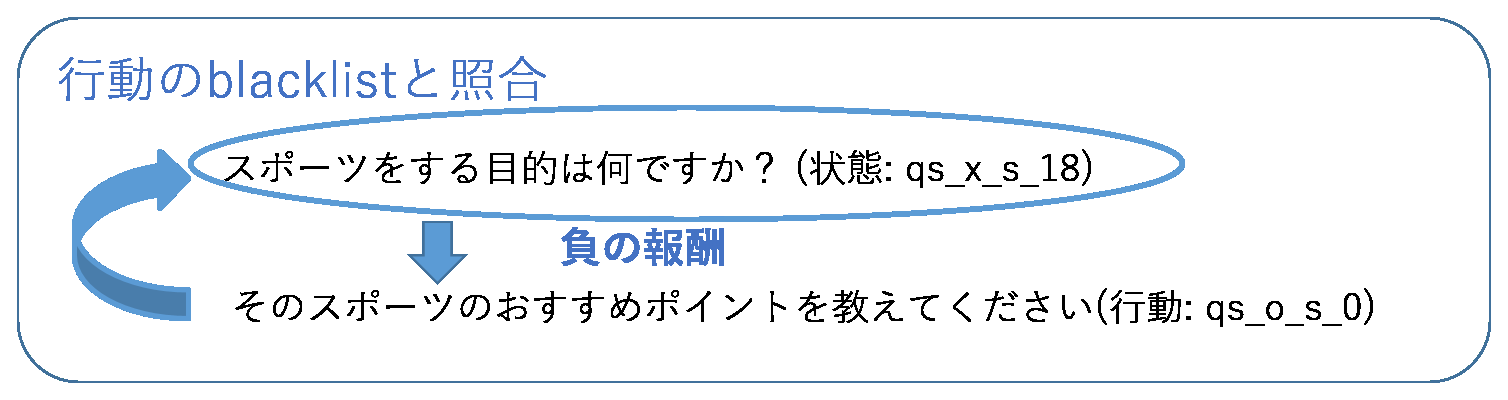
\includegraphics[width=12cm]{hosyuimage1_2.eps}
    \caption{パターン1,2に対応する報酬の付け方の例} %タイトルをつける
    \label{hosyuimage1} %ラベルをつけ図の参照を可能にする
  \end{center}
\end{figure}

\begin{figure}[tb]
  \begin{center} %センタリングする
    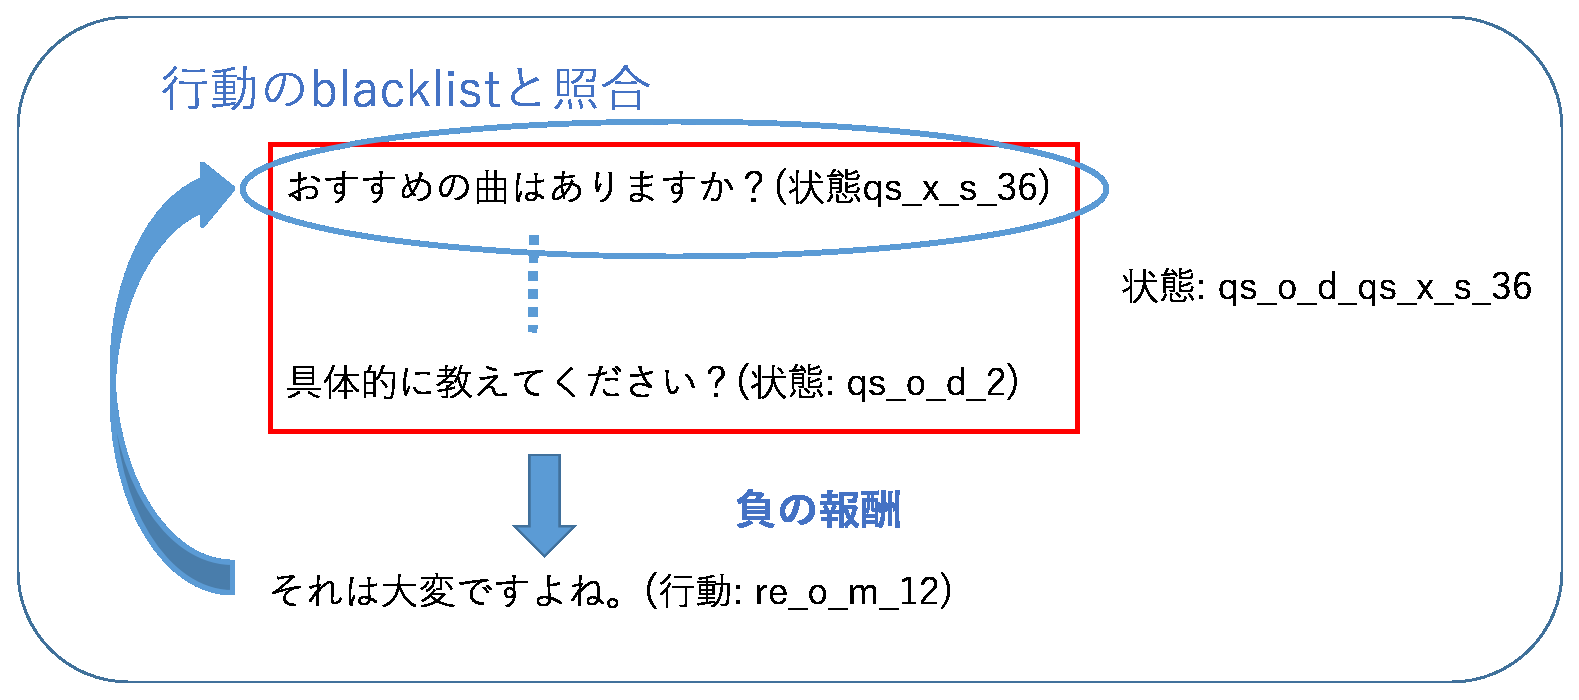
\includegraphics[width=12cm]{hosyuimage2_2.eps}
    \caption{パターン3に対応する報酬の付け方の例} %タイトルをつける
    \label{hosyuimage2} %ラベルをつけ図の参照を可能にする
  \end{center}
\end{figure}

\begin{table}[tb]
    \caption{blacklistの例(パターン1,2)}\label{blacklist1}
    \centering
    \begin{tabular}{|l|l|l|l|}\hline 
         行動&blacklist\_1(状態)&blacklist\_2(状態)&blacklist\_3(状態) \\ \hline \hline
        qs\_o\_s\_0&qs\_x\_s\_18&・・・&・・・ \\ \hline
    \end{tabular}
\end{table}

\begin{table}[tb]
    \caption{blacklistの例(パターン3)}\label{blacklist2}
    \centering
    \begin{tabular}{|l|l|l|l|}\hline 
         行動&blacklist\_1(状態)&blacklist\_2(状態)&blacklist\_3(状態) \\ \hline \hline
        re\_o\_m\_12&qs\_x\_s\_36&・・・&・・・ \\ \hline
    \end{tabular}
\end{table}


%%%%% 4章 %%%%%%%%%%%%%%%%%%%%%%%%%%%%%%%%%%%%%%%%%%%%%%%%%%%%%%%%%%%%%%%
\chapter{評価実験}
本章では提案手法を用いたシステムについて,2つのベースラインと比較し,計算量と破綻の生じにくさの2つの観点から評価を行った.
\ref{jikkenjyoken}節では全ての手法に共通する実験条件について述べる.
\ref{baseline}節では比較対象のベースライン手法の設計と実装の詳細,比較によって示したい要素について述べる.
\ref{teianjissou}節では,今回の実験での,提案手法の実装の詳細について述べる.
\ref{hatanhindo}節ではそれぞれの手法を用いて学習したモデルで実際に対話を行った結果を,一定の基準に沿って破綻にアノテートし,破綻の生じにくさを比較した.
\ref{keisanryo}節ではそれぞれの手法に関して,Qテーブルのサイズに応じたエピソード数での学習時間を比較した.

\section{共通する実験条件}\label{jikkenjyoken}
2つのベースラインシステムと提案手法では,発話集合と学習方法に関して共通したものを用いる.

発話集合として,雑談対話コーパスHazumi1902\cite{hazumi}から抜粋した117個の発話に話題変更の発話を4個加えた121個を扱う.具体的な内容は,話題「スポーツ」「音楽」「食事」「旅行」の4つの話題で用いられる発話に,どの話題にも用いられる「default」の発話を加えたものである.

学習方法は,式\ref{Q}によってある状態である行動をとる価値(Q値)を更新していくQ学習を用いた.パラメータ設定は,学習率$\alpha$を0.1,割引率$\gamma$を0.9とした.
また,システム発話とユーザ発話のセットを1交換と呼び,1エピソードを10交換として学習を行った.
エピソードは必ずシステムの話題提供の発話である「(話題)の話をしましょう」から始まる.話題は「スポーツ」「音楽」「食事」「旅行」からランダムで選択され,そのエピソード内では他の話題の発話は選択しない.1エピソード10交換が終了すると,再びシステムの話題提供から対話が始まり,これを定めたエピソード数分繰り返して学習を行う.
エピソード数は,ベースライン手法1を基準に,おおよそQテーブルのサイズ(状態数$\times$行動数)に比例するものとした.



\section{2つのベースライン手法の設計}\label{baseline}

2つのベースライン手法においては,対話の際の学習済みQテーブルを用いた発話選択において,共通した方法を用いた.具体的には,ある状態での各行動のQ値を取得し,それらをsoftmax関数(式\ref{softmax})にかけて,出力された確率から行動を確率的に選択する.

以下にベースライン手法それぞれに特有の設計を示す.

\begin{equation}\label{softmax}
y_i = \frac{e^{x_i}}{\sum_{k=1}^n e^{x_k}}   (i=1,2,\cdot\cdot\cdot,n)
\end{equation}

\subsection{発話集合を対話行為に分類して行動とする手法}
一つ目のベースライン手法は,システム発話集合を対話行為に分類して行動とする手法である.

この手法と提案手法を比較することで,状態や行動の詳細化による提案手法の破綻の生じやすさへの影響を検証する.

状態,行動は\ref{baseline2}節に示した通りであり,状態数は24,行動数は8であった.
状態数$\times$行動数は192であるため,Qテーブルのサイズは192となった.
エピソード数は1000で学習を行った.

%報酬設計
報酬設計は以下の通りである.
\begin{enumerate}
    \item ユーザ心象値(単一)($+1$, $0$, $-1$)
    \item ユーザ心象値(連続)(+5, 0, $-5$)
    \item 簡易的なシステム対話行為の連続性 (+0 ~ +10)
    \item 特定の名詞を含むユーザ発話に対するシステム行動 (+10, 0, $-10$)
    \item システム行動「thank」の選択 (0, +10)
\end{enumerate}



ユーザ心象値(単一)の報酬では,状態であるユーザの心象が低ければ$-1$,高ければ+1の報酬をつける.
ユーザ心象値(連続)の報酬では,ユーザの心象が3連続で高ければ+5,低ければ$-5$の報酬をつける.
これらユーザ心象に関する報酬は,システムがユーザの心象がより高くなる行動を選択するために設計されている.

簡易的なシステム対話行為の連続性への報酬は,簡易対話行為の連続性に人手で+1から+10の報酬をつける.
報酬の付け方を表\ref{hosyu3}に示す.
表の左側がターン$t-1$の簡易対話行為を表しており,そこからターンtで上側の簡易対話行為が選ばれたときの報酬が示されている.
この報酬は,質問をした後に応答を返すような流れは自然であるが,応答を返した後にもう一度応答を返すのは不自然であるというような,簡易対話行為レベルでの自然さを表現している.

特定の名詞を含むユーザ発話に対するシステム行動への報酬では,ユーザ発話に特定名詞(固有名詞等)が含まれる場合に,指示語ありの対話行為を選べば+10,含まれない場合に選べば$-10$の報酬をつける.
この報酬は指示語が適切なタイミングで使われるように設計されている.

システム行動「thank」の選択への報酬は,話題変更の前に感謝の対話行為が選ばれた場合,+10の報酬をつける.
この報酬は感謝の対話行為は,一つの話題が終わるときに付けるのが適切であるという考えのもと,設計されている.


\begin{table}[tb]
    \caption{簡易的なシステム対話行為の連続性への報酬}\label{hosyu3}
    \centering
    \begin{tabular}{|l|l|l|l|l|}\hline 
         $t-1\backslash t$&質問&応答&情報提供 \\ \hline 
         質問&3&3&4 \\ \hline
         応答&5&1&4 \\ \hline
         情報提供&9&1&0 \\ \hline
         話題変更&10&0&0 \\ \hline
    \end{tabular}
\end{table}



\subsection{発話全てを行動とする手法}
二つ目のベースライン手法は,システム発話集合中の発話をそのまま状態,行動とするものである.

この手法と提案手法を比較することで,提案手法の計算量削減への有効性と,状態数や行動数削減による破綻の生じやすさへの影響を検証する.

状態と行動は発話集合中の発話全てであるが,話題変更の4発話はエピソードの最初に提示して,それ以降は選択しないものとしたため,行動には含めないこととした.
状態数が121,行動数が117となるため,Qテーブルのサイズは14157であった.
ベースライン手法1とのQテーブルのサイズの比例関係を考えて,この手法ではエピソード数76000で学習を行った.

報酬としては,提案手法と同様に,まず各行動に,この発話の後に来てはいけないという発話集合(blacklist)を設ける.
次に,行動が選択されたときに,その前のシステム発話が,その行動のblacklist内にあれば$-20$の報酬を与える.





\section{計算量を考慮した行動設計に基づく手法の実装}\label{teianjissou}
提案手法における行動と報酬の設計は,\ref{jyotaikodo}節に示した,ベースライン手法1の対話行為を一部詳細化したものである.状態数が113,行動数が51であるため,Qテーブルのサイズは5763となった.ベースライン手法1とのQテーブルのサイズの比例関係を考えて,提案手法ではエピソード数30000で学習を行った.

報酬に関しては,\ref{hosyu}節に示したものであるが,ベースライン手法2と同様に,与える負の報酬の値を一律$-20$に設定した.

学習済みQテーブルを用いた対話での発話選択では,学習したQテーブルと,ベースライン手法1での学習済みQテーブルの両方を用いる.
まず,ベースライン手法1の状態を取得し,その学習済みQテーブルを用いて,対話行為を選択する.
次に,本章で述べた提案手法での状態を取得し,その状態での各行動のQ値を取得する.
Q値を取得した行動の中で,選択した対話行為に属するもののみを取り出す.
取り出された行動のQ値を正規化し,softmax関数(式\ref{softmax})にかけることで,その行動の選択確率を決定し,行動選択を行う.

発話選択の全体像の例は図\ref{hatuwasentakuzu}のようになる.
まず,「最近はまっている食べ物はありますか?」というシステム発話と,それに対する「バナナにはまっています」というユーザ発話,入力された心象の組み合わせから状態が取得される.その状態をもとに,対話行為を行動とする手法によってre\_o\_mという対話行為が選択されたとする.
一方,提案手法側では,「最近はまっている食べ物はありますか?」という発話を状態として,その状態での行動(発話)全てのQ値が取得される.
例では,これらの行動(発話)の中で,re\_o\_mに属しており,Q値の高い「とても美味しそうですね」が確率的に選択されている.

\begin{figure}[ht]
  \begin{center} %センタリングする
    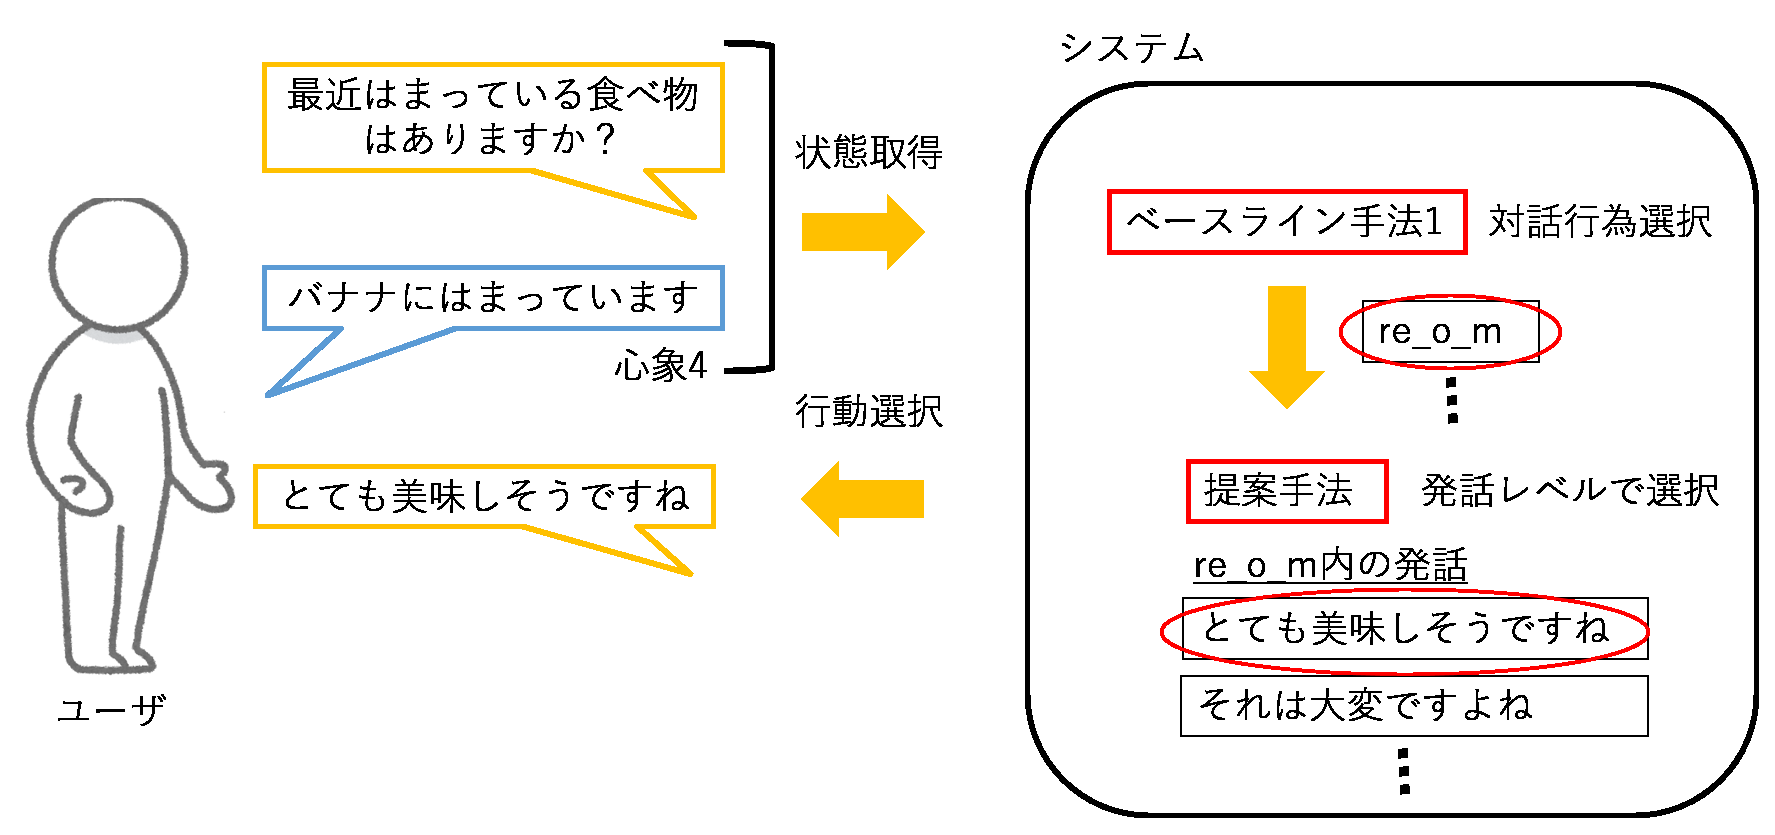
\includegraphics[width=\linewidth]{hatuwasentaku.eps}
    \caption{発話選択方法} %タイトルをつける
    \label{hatuwasentakuzu} %ラベルをつけ図の参照を可能にする
  \end{center}
\end{figure}


\section{破綻の生じにくさに関する評価}\label{hatanhindo}
本節では提案手法の設計が破綻削減に有効であることを示す.
そのため,提案手法及びベースライン手法2つの学習済みQテーブルを用いてテキスト対話を行い,生じた破綻の数を比較して,破綻の生じやすさの評価を行った.

テキスト対話は,システム発話とユーザ発話の組み合わせを1交換として,10交換1セットで行った.話題「スポーツ」「音楽」「食事」「旅行」の4つに関して5セットずつ計20セット200交換を評価の対象とした.
特定話題に関する対話では,その特定話題の発話とdefault発話が全体の発話集合となり,発話はその中から選択される.

評価は東中らの研究\cite{higashinaka}で用いられた破綻の基準をもとに行った.
以下の基準をもとに各交換に対して〇△×でアノテーションをつけた.
\begin{itemize}
\item 〇破綻ではない: \\当該システム発話のあと対話を問題
無く継続できる.
\item △破綻と言い切れないが,違和感を感じる発話:\\当該
システム発話のあと対話をスムーズに継続することが困難.
\item ×あきらかにおかしいと思う発話. 破綻: \\当該システ
ム発話のあと対話を継続することが困難.
\end{itemize}
△や×の数と,全交換数に対する△や×の割合によって破綻の生じやすさの評価を行った.
また,東中らの研究\cite{higashinaka}によると,これらのアノテーション基準では,△と×の付け方が個人によってばらつきが大きい.
そのため,△と×の和も算出し,同様に評価を行った.

ベースライン手法と提案手法の比較を表\ref{hatanhindohyo1}と\ref{hatanhindohyo2}に基づいて説明する.表\ref{hatanhindohyo1}を見ると,ベースライン手法1では△の数が21個,×の数が13個であるのに対して,提案手法では△の数が4個,×の数が6個と減少している.また,それぞれの全交換数に対する割合も△では11\%から2\%,×では6.5\%から3\%とかなり減少している.また,\ref{hatanhindohyo2}を見ると,提案手法では△と×の数が24個減っていて.割合も17\%から5\%となっていて,全体的にも違和感のある発話はかなり減っている.

また,ベースライン手法2と提案手法の比較を表\ref{hatanhindohyo1}と表\ref{hatanhindohyo2}に基づいて説明する.
表\ref{hatanhindohyo1}を見ると,ベースライン手法2では△の数が8個,×の数が5個であるのに対して,提案手法では△の数が4個,×の数が6個となっていて,△の数は多少減っているが,×の数は多少増えている.また,それぞれの全交換数に対する割合も同様である.また,\ref{hatanhindohyo2}を見ると,提案手法では△と×の数が3個減っていて,割合も6.5\%から5\%となっている.これらはほぼ同程度であるとみなせる.

これらのことから,提案手法の設計が破綻の削減に有効であることが分かった.



\begin{table}[tb]
\caption{〇と△と×による破綻の生じやすさの比較}\centering\label{hatanhindohyo1}
  \begin{tabular}{|l|l|l|l|l|l|} \hline
     & 〇& △& ×& △の割合(\%) &×の割合(\%) \\ \hline \hline
    提案手法 & 190 & 4 & 6 &2\% &3\%  \\ \hline
    ベースライン手法1 & 166 & 21 & 13 & 11\% & 6.5 \\ \hline
    ベースライン手法2 &  187&  8& 5& 4\% &2\% \\ \hline
  \end{tabular}
\end{table}
\begin{table}[tb]
\caption{〇と△×による破綻の生じやすさの比較}\centering\label{hatanhindohyo2}
  \begin{tabular}{|l|l|l|l|} \hline
     & 〇& △と×&△と×の割合(\%)\\ \hline \hline
    提案手法 & 190 & 10 &5.0\% \\ \hline
    ベースライン手法1 & 166 & 34 &  17\% \\ \hline
    ベースライン手法2 &  187&  13 & 6.5\% \\ \hline
  \end{tabular}
\end{table}

以下で提案手法での,破綻改善への設計の有効性について述べる.
\ref{bunseki}節での,パターン1から3の破綻について,ベースライン手法1で生じた破綻例と,提案手法での改善例を示し,提案手法の設計との関連を述べる.

\subsection*{パターン1の破綻改善}
ベースライン手法1では,パターン1の破綻と同様の破綻が生じた.
図\ref{baseline2pattern1}を見ると,指示語なし質問(qs\_x\_s)に対して,不適切な指示語あり質問(qs\_o\_s)が選択されたことで破綻が生じている.
この例では,S1で旅行の目的を聞いており,U1でユーザが旅行の目的について答えることが予測できる.
それにも関わらず,S2で「その旅先」と具体的な旅先について尋ねているため,破綻が生じている.

一方,提案手法では,パターン1の破綻に関する改善が見られた.
同じ例ではないが,図\ref{teianpattern1}を見ると,指示語なし質問(qs\_x\_s)に対して,適切な指示語あり質問(qs\_o\_s)を選択することができている.
この例では,S1で好きなスポーツについて尋ね,ユーザは何らかのスポーツを答えることが予測される.S2では特定のスポーツをテレビで観戦するかを尋ねており,これは破綻の生じない発話となっている.

このような破綻の生じない発話を選択できた理由として,提案手法での,対話行為の詳細化と,システム発話の内容的整合性への報酬が有効に働いていることが挙げられる.
S2で選択された「そうですか。テレビでの観戦はされるんですか?」という発話は,指示語あり質問(特定話題)が詳細化された,qs\_o\_s\_0という行動である.また,S1での「好きなスポーツはなんですか」という発話は,指示語なし質問が詳細化された,qs\_x\_s\_20という状態として取得されている.報酬設計では,qs\_o\_s\_0という行動のblacklistにはqs\_x\_s\_20という状態を入れていなかったが,他の不適切な指示語なし質問の発話(状態)はblacklistに入れていた.
これにより,相対的に「そうですか。テレビでの観戦はされるんですか?」という,破綻の生じない発話が選ばれやすくなるように学習されたと考えられる.

\begin{figure}[tb]
\centering
\begin{screen}
\begin{Verbatim}[commandchars=\\\{\}]
S1:  旅行に行くときはなにか目的はありますか?(qs_x_s)
U1: 美しい景色を見ることですかね
\mychangecolor{S2(破綻): その旅先で何かハプニングはありましたか!(qs_o_s)
}
U2: どの?
\end{Verbatim}
\end{screen}
\caption{ベースライン手法1でのパターン1の破綻例}
\label{baseline2pattern1}
\end{figure}

\begin{figure}[htb]
\centering
\begin{screen}
\begin{Verbatim}[commandchars=\\\{\}]
S1:  好きなスポーツはなんですか?(状態: qs_x_s_20)
U1: 野球です
\mychangecolor{S2: そうですか。テレビでの観戦はなされるんですか?(行動: qs_o_s_0)
}
U2: ええ主にテレビで見ます
\end{Verbatim}
\end{screen}
\caption{提案手法でのパターン1の破綻改善}
\label{teianpattern1}
\end{figure}

\subsection*{パターン2の破綻改善}
ベースライン手法1では,パターン2の破綻と同様の破綻が生じた.
図\ref{baseline2pattern2}を見ると,指示語なし質問(qs\_x\_s)に対して,不適切な指示語あり応答(re\_o\_m)が選択されたことで破綻が生じている.
この例では,S1でスイーツを買う場所について聞いており,U1でユーザがその場所について答えることが予測できる.
それにも関わらず,S2で「面白い」という反応を返しているため,違和感を感じる発話になっている.

一方,提案手法では,パターン2の破綻に関する改善が見られた.
ベースライン手法1と同様の例で,図\ref{teianpattern2}を見ると,指示語なし質問(qs\_x\_s)に対して,適切な指示語あり応答を返すことができている.この例では,同様の質問に対して,「いいですね,とても興味深いです!」という破綻の生じない発話を返している.

このような破綻の生じない発話を選択できた理由として,提案手法での,対話行為の詳細化と,システム発話の内容的整合性への報酬が有効に働いていることが挙げられる.S2で選択された「いいですね,とても興味深いです!」という発話は,指示語あり応答が詳細化された,re\_o\_m\_11という行動である.また,S1での「ちょっと特別なスイーツを買うときは~」という発話は,指示語なし質問が詳細化された,qs\_x\_s\_24という状態として取得されている.報酬設計では,re\_o\_m\_11という行動のblacklistにはqs\_x\_s\_24という状態を入れていなかったが,他の不適切な指示語なし質問の発話(状態)はblacklistに入れていた.これにより,相対的に「いいですね.とても興味深いです!」という,破綻の生じない発話が選ばれやすくなるように学習されたと考えられる.




\begin{figure}[tb]
\centering
\begin{screen}
\begin{Verbatim}[commandchars=\\\{\}]
S1: ちょっと特別なスイーツを買うときは近くのお店とか
    「デパートの地下」とか、利用しますか?(qs_x_s)
U1: やはりコンビニですね
\mychangecolor{S2(破綻): 面白いですよね(re_o_m)}
U2: 面白いかな
\end{Verbatim}
\end{screen}
\caption{ベースライン手法1でのパターン2の破綻例}
\label{baseline2pattern2}
\end{figure}

\begin{figure}[tb]
\centering
\begin{screen}
\begin{Verbatim}[commandchars=\\\{\}]
S1: ちょっと特別なスイーツを買うときは近くのお店とか
    「デパートの地下」とか、利用しますか?(状態: qs_x_s_24)
U1: やはりコンビニですね
\mychangecolor{S2:  いいですね,とても興味深いです!(行動: re_o_m_11)}
U2: そうですか
\end{Verbatim}
\end{screen}
\caption{提案手法でのパターン2の破綻改善}
\label{teianpattern2}
\end{figure}

\subsection*{パターン3の破綻改善}
ベースライン手法1では,今回の実験でも,パターン3の破綻と同様の破綻が生じた.図\ref{baselinepattern3}を見ると,defaultの指示語あり質問(qs\_o\_d)に対して,不適切な指示語あり応答(re\_o\_m)が選択されたことで破綻が生じている.
この例では,S1で甘いものと辛いもののどっちが好きかを尋ねていて,続いてS2でその具体例について尋ねる形になっている.ここではユーザが甘いものか辛いものかの具体例を答えることが予測されるが,S3で「すごい」という反応を返しているため,破綻が生じている.

一方,提案手法では,パターン3の破綻に関する改善が見られた.同じ例ではないが,図\ref{teianpattern3}を見ると,defaultの指示語あり質問(qs\_o\_d)に対して,適切な指示語あり応答を返すことができている.この例では,S1でカラオケで歌う曲について尋ね,続いてその具体例について尋ねる形になっている.S3では「そうなんですか~」という破綻の生じない発話を返している.

このような破綻の生じない発話を選択できた理由として,提案手法での,対話行為の詳細化と,システム発話の内容的整合性への報酬が有効に働いていることが挙げられる.S3で選択された「そうなんですね。新しい知識が~」という発話は,指示語あり応答が詳細化された,re\_o\_m\_17という行動である.また,S1で選択された「カラオケでよくなにをうたうのですか?」という発話と,S2で選択された「具体的にはどういったものですか」という発話の組み合わせは,qs\_o\_d\_qs\_x\_s\_16という状態として取得されている.報酬設計では,re\_o\_m\_17という行動のblacklistにはqs\_o\_d\_qs\_x\_s\_16という状態を入れていなかったが,他の不適切な指示語なし質問と指示語あり質問(default)の組み合わせの状態はblacklistに入れていた.
これにより,相対的に「そうなんですか~」という破綻の生じない発話が選ばれやすくなるように学習されたと考えられる.





\begin{figure}[tb]
\centering\label{baselinepattern3}
\begin{screen}
\begin{Verbatim}[commandchars=\\\{\}]
S1: 甘いものと、からいものどちらがお好きですか?(qs_x_s)
U1: 甘い物です
S2: 具体的には教えてもらえますか?(qs_o_d)
U2: チョコとかですかね
\mychangecolor{S3(破綻): すごい!(re_o_m)}
U3: すごいかな
\end{Verbatim}
\end{screen}
\caption{ベースライン手法1でのパターン3の破綻例}
\end{figure}

\begin{figure}[tb]
\centering\label{teianpattern3}
\begin{screen}
\begin{Verbatim}[commandchars=\\\{\}]
S1: カラオケでよくなにをうたうのですか?(状態: qs_x_s_16)
U1: やはりスピッツですね
S2: 具体的にはどういったものですか?(状態: qs_o_d_qs_x_s_16)
U2: チェリーとかロビンソンとかです
\mychangecolor{S3: そうなんですね。新しい知識が増えました。}
    \mychangecolor{私も一度聞いてみたいと思います!(行動: re_o_m_17)}
U3: ええぜひ
\end{Verbatim}
\end{screen}
\caption{提案手法でのパターン3の破綻改善}
\end{figure}

\section{計算量に関する評価}\label{keisanryo}
本節では,提案手法の設計が計算時間の削減に有効であることを示す.
本実験では,提案手法,ベースライン手法1,ベースライン手法2に関して学習を行った際の計算時間を比較した.
それぞれのQテーブルのサイズ,エピソード数,学習にかかる総計算時間,1エピソード当たりの計算時間を表\ref{keisanryohyo}に示す.
これらを用いてQテーブルのサイズによるエピソード数の変化,また,エピソード数の変化による計算時間の変化,手法の設計が計算時間に与える影響等について考察する.
また,\ref{hatanhindo}節で示した破綻の生じにくさと総計算時間両方について考慮することで,手法の総合的な性能を述べる.
提案手法に関しては,破綻の生じにくさの実験において,提案手法とベースライン手法1両方の学習済みQテーブルを用いて発話選択を行った.
そのため,提案手法の性能に関しては,提案手法とベースライン手法1両方の学習の成果であると言える.
ゆえに,表\ref{keisanryohyo}の提案手法のQテーブルのサイズやエピソード数,計算時間には,ベースライン手法1の値を足し合わせたものを記述している.

提案手法とベースライン手法1の比較を表\ref{keisanryohyo}に基づいて説明する.
まず,提案手法とベースライン手法1の1エピソード当たりの計算時間を比べると,ベースライン手法1が提案手法の約1.4倍程度になった.
これは,提案手法に比べて,ベースライン手法1ではプログラム上で最も時間のかかる報酬を与える部分で,与える報酬の種類が多く,参照する状態や行動が多いことに起因する.また,提案手法ではベースライン手法1(対話行為を行動とする手法)の対話行為を詳細化して状態と行動を設計している.そのため,Qテーブルに関しては,提案手法がベースライン手法1の約31倍になっている.今回の実験では,学習するエピソード数をQテーブルにサイズに比例するものとしたため,提案手法では,エピソード数が,ベースライン手法1の約31倍になっている.
これらのことから,総計算時間に関して,提案手法がベースライン手法1の約21倍となっている.

提案手法とベースライン手法1の,計算時間と破綻の生じにくさの関係について述べる.
本実験と同じ条件で学習されたQテーブルを用いて対話を行った,\ref{hatanhindo}節の破綻の生じにくさに関する評価実験では,提案手法とベースライン手法1では,提案手法手法が優れていることが示された.
また,本実験では,提案手法の総計算時間はベースライン手法1の約21倍であった.
これらのことから,提案手法は,計算時間は増えるが,破綻の生じにくさに関して,ベースライン手法1よりも優れた性能を持つ手法といえる.

提案手法とベースライン手法2の比較を表\ref{keisanryohyo}に基づいて説明する.
まず,提案手法とベースライン手法2の1エピソード当たりの計算時間を比べると,提案手法がやや多いものの,ほぼ同じとみなせる程度であった.
これは,提案手法とベースライン手法2では,プログラム上で最も時間のかかる報酬を与える部分の設計がほぼ同じであることが原因であると考えられる.
また,提案手法ではベースライン手法1(対話行為を行動とする手法)で破綻の生じやすい対話行為のみを詳細化して状態と行動の設計に用いている.一方,ベースライン手法2では,全ての発話を状態と行動の設計に用いている.これによってベースラインライン手法2ではQテーブルのサイズが大きく,提案手法の約2.4倍になっており,エピソード数も約2.4倍になっている.
1エピソード当たりの計算時間があまり変わらないことと,学習するエピソード数が
ベースライン手法2では約2.4倍であることから,総計算時間に関してもベースライン手法は約2.2倍程度になっている.

提案手法とベースライン手法2の計算時間と破綻の生じにくさの関係について述べ,提案手法が計算時間の削減に有効であることを示す.
本実験と同じ条件で学習されたQテーブルを用いて対話を行った,\ref{hatanhindo}節の破綻の生じにくさに関する評価実験では,提案手法とベースライン手法2は破綻の生じにくさに関して,同程度の性能を持つことが示された.
また,本実験では,ベースライン手法の総計算時間は提案手法の約2.2倍であった.
これらのことから,提案手法では,約2.2倍の計算時間がかかるベースライン手法2と比べて,破綻の生じにくさに関して同程度の性能を実現できているといえる.
よって,提案手法の設計は計算時間の削減に有効であることが示された.

\begin{table}[tb]
    \caption{計算時間の比較}\label{keisanryohyo}
    \scriptsize
    \centering
    \begin{tabular}{|l|l|l|l|l|}\hline 
         &Qテーブルのサイズ&エピソード数&総計算時間&計算時間(1エピソード)  \\ \hline 
         提案手法&5955&31000&2777秒&0.08958秒 \\ \hline
         ベースライン手法1&192&1000&130秒&0.130秒 \\ \hline
         ベースライン手法2&14157&76000&6118秒&0.08050秒 \\ \hline
    \end{tabular}
\end{table}

\begin{table}[tb]
    \caption{計算時間の比較}\label{keisanryohyo}
    \scriptsize
    \centering
    \begin{tabular}{|l|l|l|l|l|}\hline 
         &Qテーブルのサイズ&エピソード数&総計算時間&計算時間(1エピソード)  \\ \hline 
         提案手法&5955&31000&2777秒&0.08958秒 \\ \hline
         ベースライン手法1&192&1000&130秒&0.130秒 \\ \hline
         ベースライン手法2&14157&76000&6118秒&0.08050秒 \\ \hline
    \end{tabular}
\end{table}\begin{table}[tb]
    \caption{計算時間の比較}\label{keisanryohyo}
    \scriptsize
    \centering
    \begin{tabular}{|l|l|}\hline 
         &総計算時間  \\ \hline 
         提案手法&2777秒 \\ \hline
         ベースライン手法1&130秒 \\ \hline
         ベースライン手法2&6118秒 \\ \hline
    \end{tabular}
\end{table}
\begin{table}[tb]
\caption{〇と△×による破綻の生じやすさの比較}\centering\label{hatanhindohyo2}
  \begin{tabular}{|l|l|l|l|} \hline
     & 〇& △と×&△と×の割合(\%)\\ \hline \hline
    提案手法 & 190 & 10 &5.0\% \\ \hline
    ベースライン手法1 & 166 & 34 &  17\% \\ \hline
    ベースライン手法2 &  187&  13 & 6.5\% \\ \hline
  \end{tabular}
\end{table}

%%%%% 5章 %%%%%%%%%%%%%%%%%%%%%%%%%%%%%%%%%%%%%%%%%%%%%%%%%%%%%%%%%%%%%%%
\chapter{結論}
本研究では,強化学習を用いた傾聴型対話システムの発話選択手法に関して,計算量を考慮した行動設計を行い,破綻の減少を目指した.
発話を対話行為に分類して状態や行動を設計する手法を分析し,破綻の生じやすい対話行為の順番を明らかにした.
提案手法では,それらの対話行為内のみを詳細化して状態や行動を設計し,連続するシステム発話の内容的整合性に基づいた報酬を設定した.

破綻の生じにくさと計算時間の2つの観点から提案手法の評価実験を行った.実験の結果,提案手法は,破綻の生じにくさの点で,対話行為を行動とする手法よりも優れており.発話全部を行動とする手法と同程度の性能であった.また,提案手法は,計算時間の点で発話全部を行動とする手法よりも優れていることが示された.




本研究では,ユーザの,話を聞いて欲しいという欲求を満たすために,ユーザが気持ちよく対話を続けられるよう破綻の少ない対話システムを目指した.
そのために,システム発話から次のユーザ発話を予測し,それに対して破綻を起こすシステム発話は選択されにくくなるよう学習を行った.
一方,ユーザ発話を予測しきれないシステム発話に関しては,一部を除いて,次にどのシステム発話が来ても破綻が起こると決め,一律に選択されにくくなるように学習した.
これにより,ユーザ発話の内容によっては破綻が起こらないにも関わらず,選択されにくいシステム発話があった.
この設計では,本来あり得たシステム発話が選択されづらくなることで,発話候補が減る.これによって,長い間,もしくは複数回対話を行うと,同じような順番での発話選択が多くなり,ユーザに飽きられやすくなってしまう.
しかし,ユーザの,話を聞いてほしいという欲求を満たすためには,ある程度長い間,もしくは複数回対話を行うことも重要である.

今後の課題としては,ユーザと長い間,もしくは複数回対話を行っても飽きられないシステムの開発が挙げられる.
これの実現方法として,ユーザの応答からも状態を取得することが挙げられる.
ユーザ応答から状態を取得することで,ユーザの応答が予測できない発話も,ユーザ状態によって選択してよいかどうかを学習できる.これにより,発話の選択肢が増え,より飽きられないシステムを実現できるのではないかと考えている.




%%%%% 参考文献 %%%%%%%%%%%%%%%%%%%%%%%%%%%%%%%%%%%%%%%%%%%%%%%%%%%%%%%%%%
{
%\footnotesize
\bibliographystyle{IEEEbib}
\bibliography{cite}
}

%%%%% 謝辞 %%%%%%%%%%%%%%%%%%%%%%%%%%%%%%%%%%%%%%%%%%%%%%%%%%%%%%%%%%%%%%
\begin{acknowledgement}
本研究の遂行に際し,多大なる御指導,御鞭撻を賜りました大阪大学産業科学研
究所 駒谷和範教授,武田龍准教授に,深く感謝いたします.
また,本研究を進めるにあたり,多くの助言を頂いた,大阪大学大学院工学研究
科電気電子情報通信工学専攻 奥野尚己氏をはじめとする大阪大学産業科学研究所 駒谷
研究室の学生一同に深く感謝いたします.
また,日頃よりお世話になりました駒谷研究室技術補佐員 谷端紀久子氏,事務補
佐員 松下美佐氏に深く感謝致します.
\end{acknowledgement}

\newpage

\appendix

\end{document}
